\chapter{Visual design}\label{ch:visualDesign}
\section{Concept art}
Concept art was created for several iterations of the player-controlled pirate characters, some of which is seen in Figure \ref{fig:pirate_concepts}. They were drawn with a simple, cartoonish look in mind, so that the characters easily catch the players' eyes. 

\begin{figure}[h!]
    \centering
    \begin{subfigure}[b]{0.2\textwidth}
        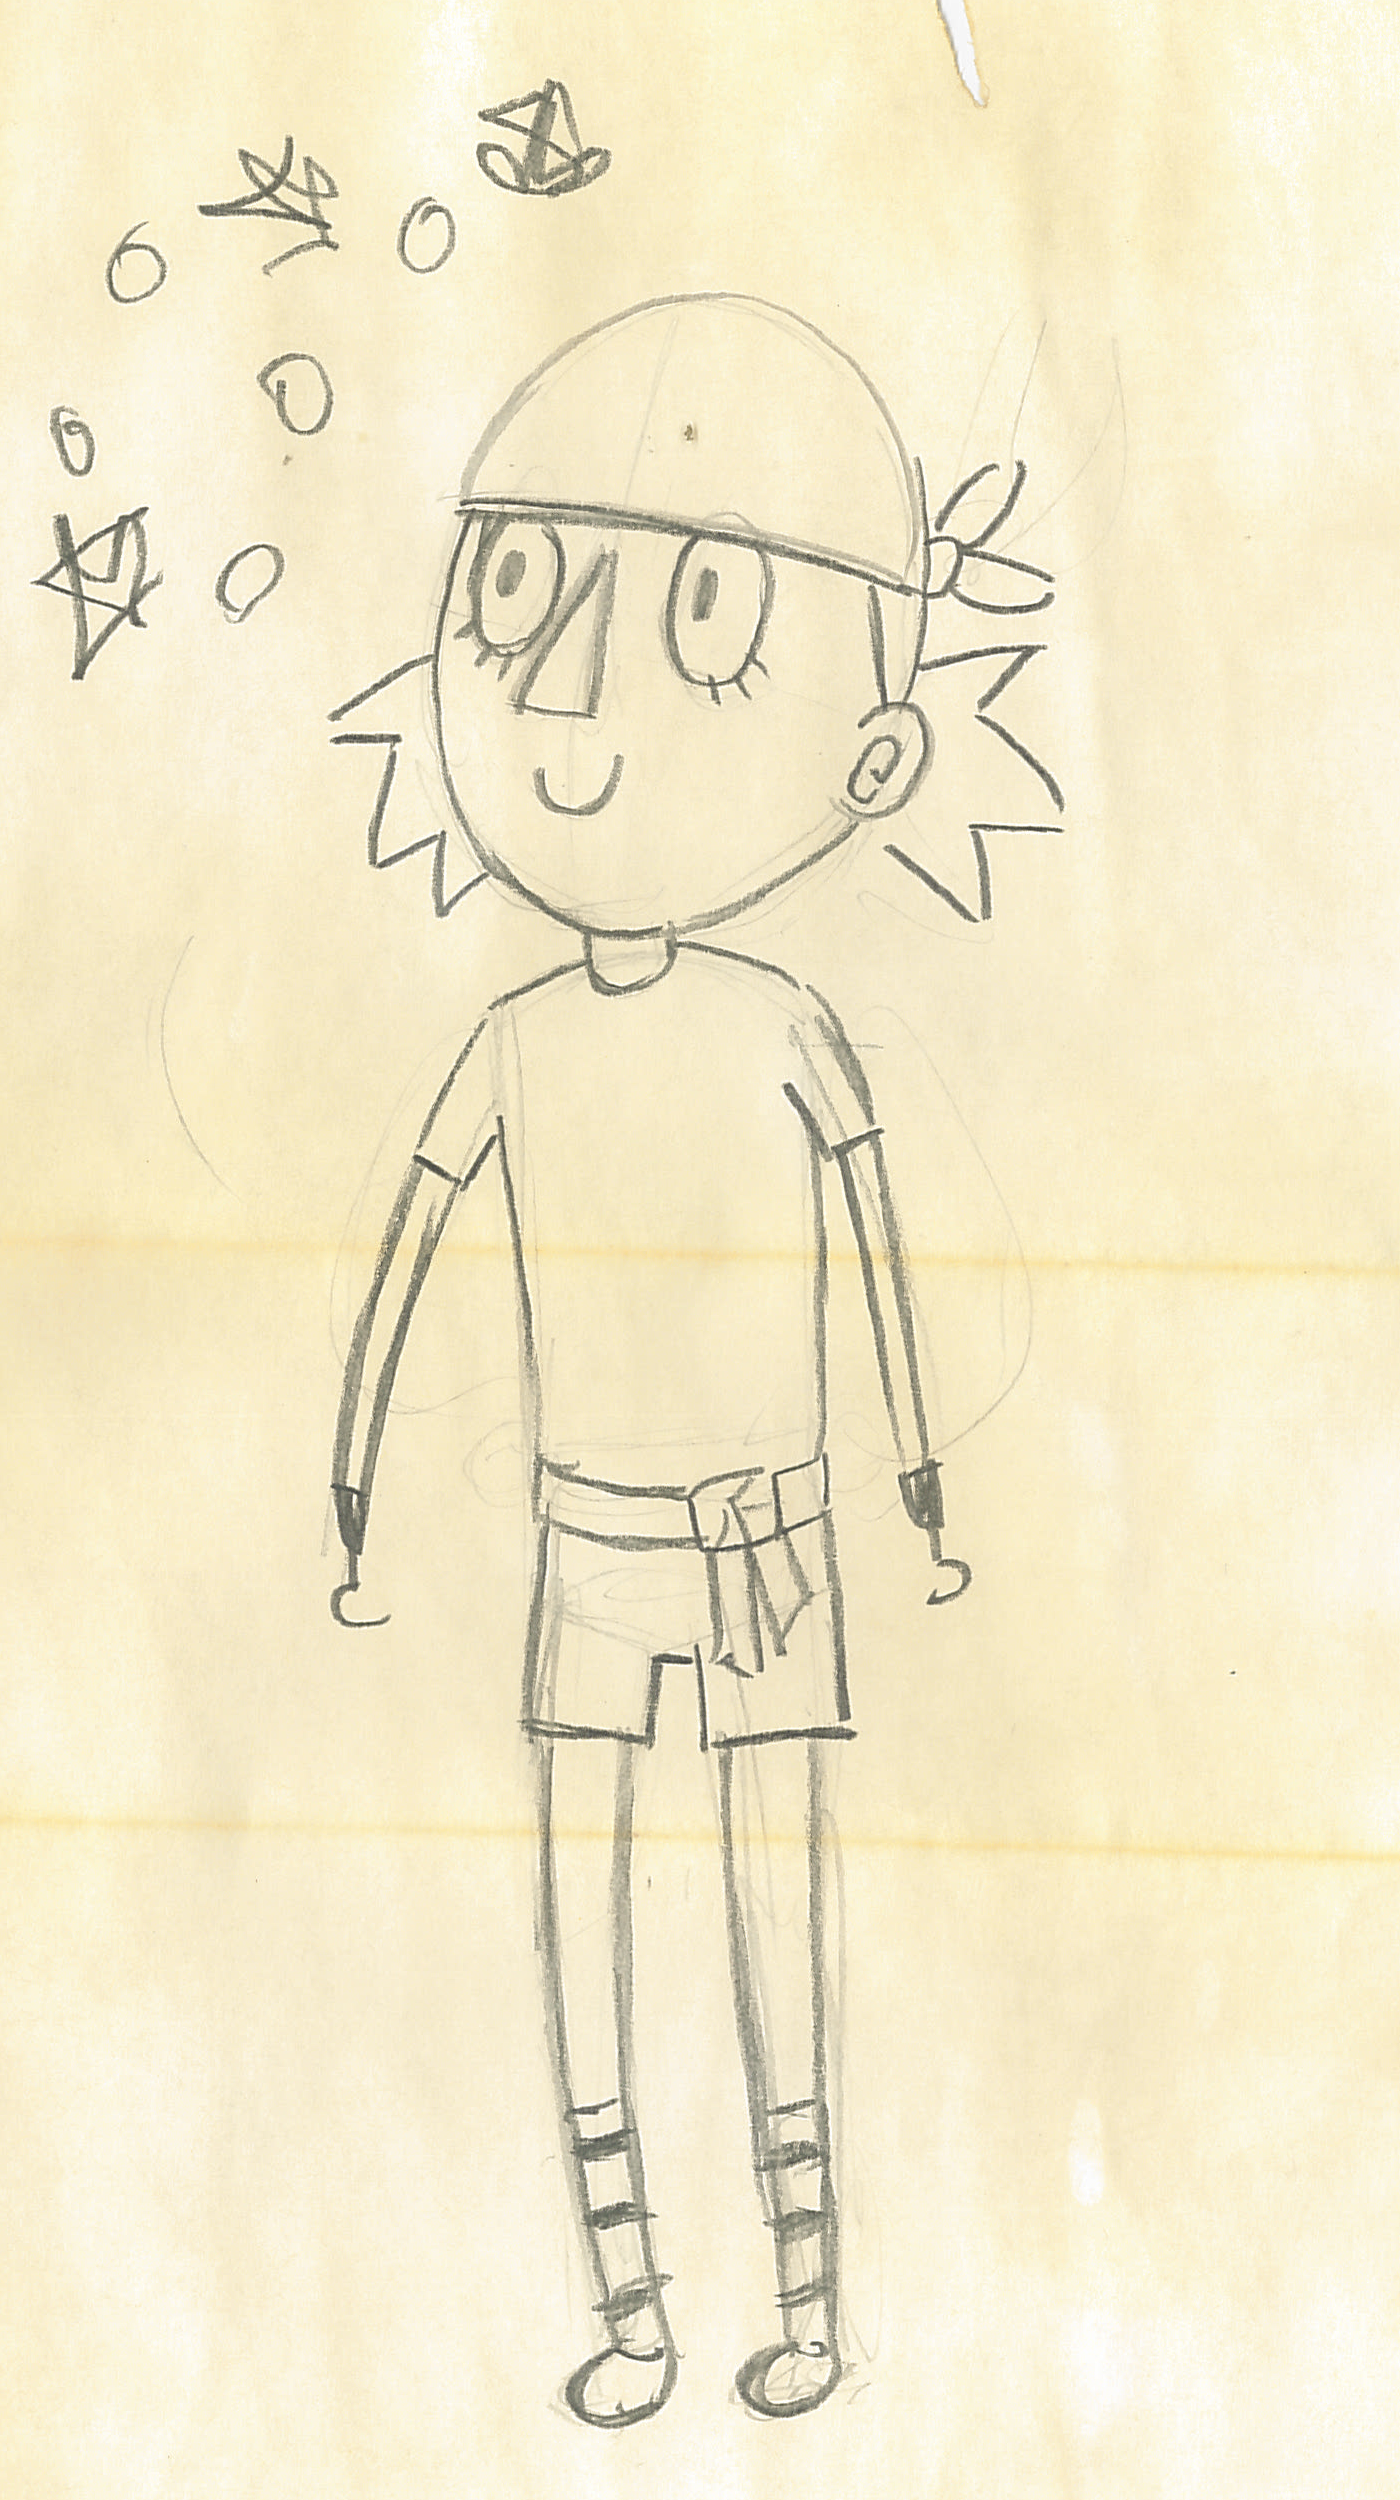
\includegraphics[width=\textwidth]{figures/pirate_concept_0.png}\caption{ \label{fig:pirate_concept_0}}
    \end{subfigure}
    \begin{subfigure}[b]{0.2\textwidth}
        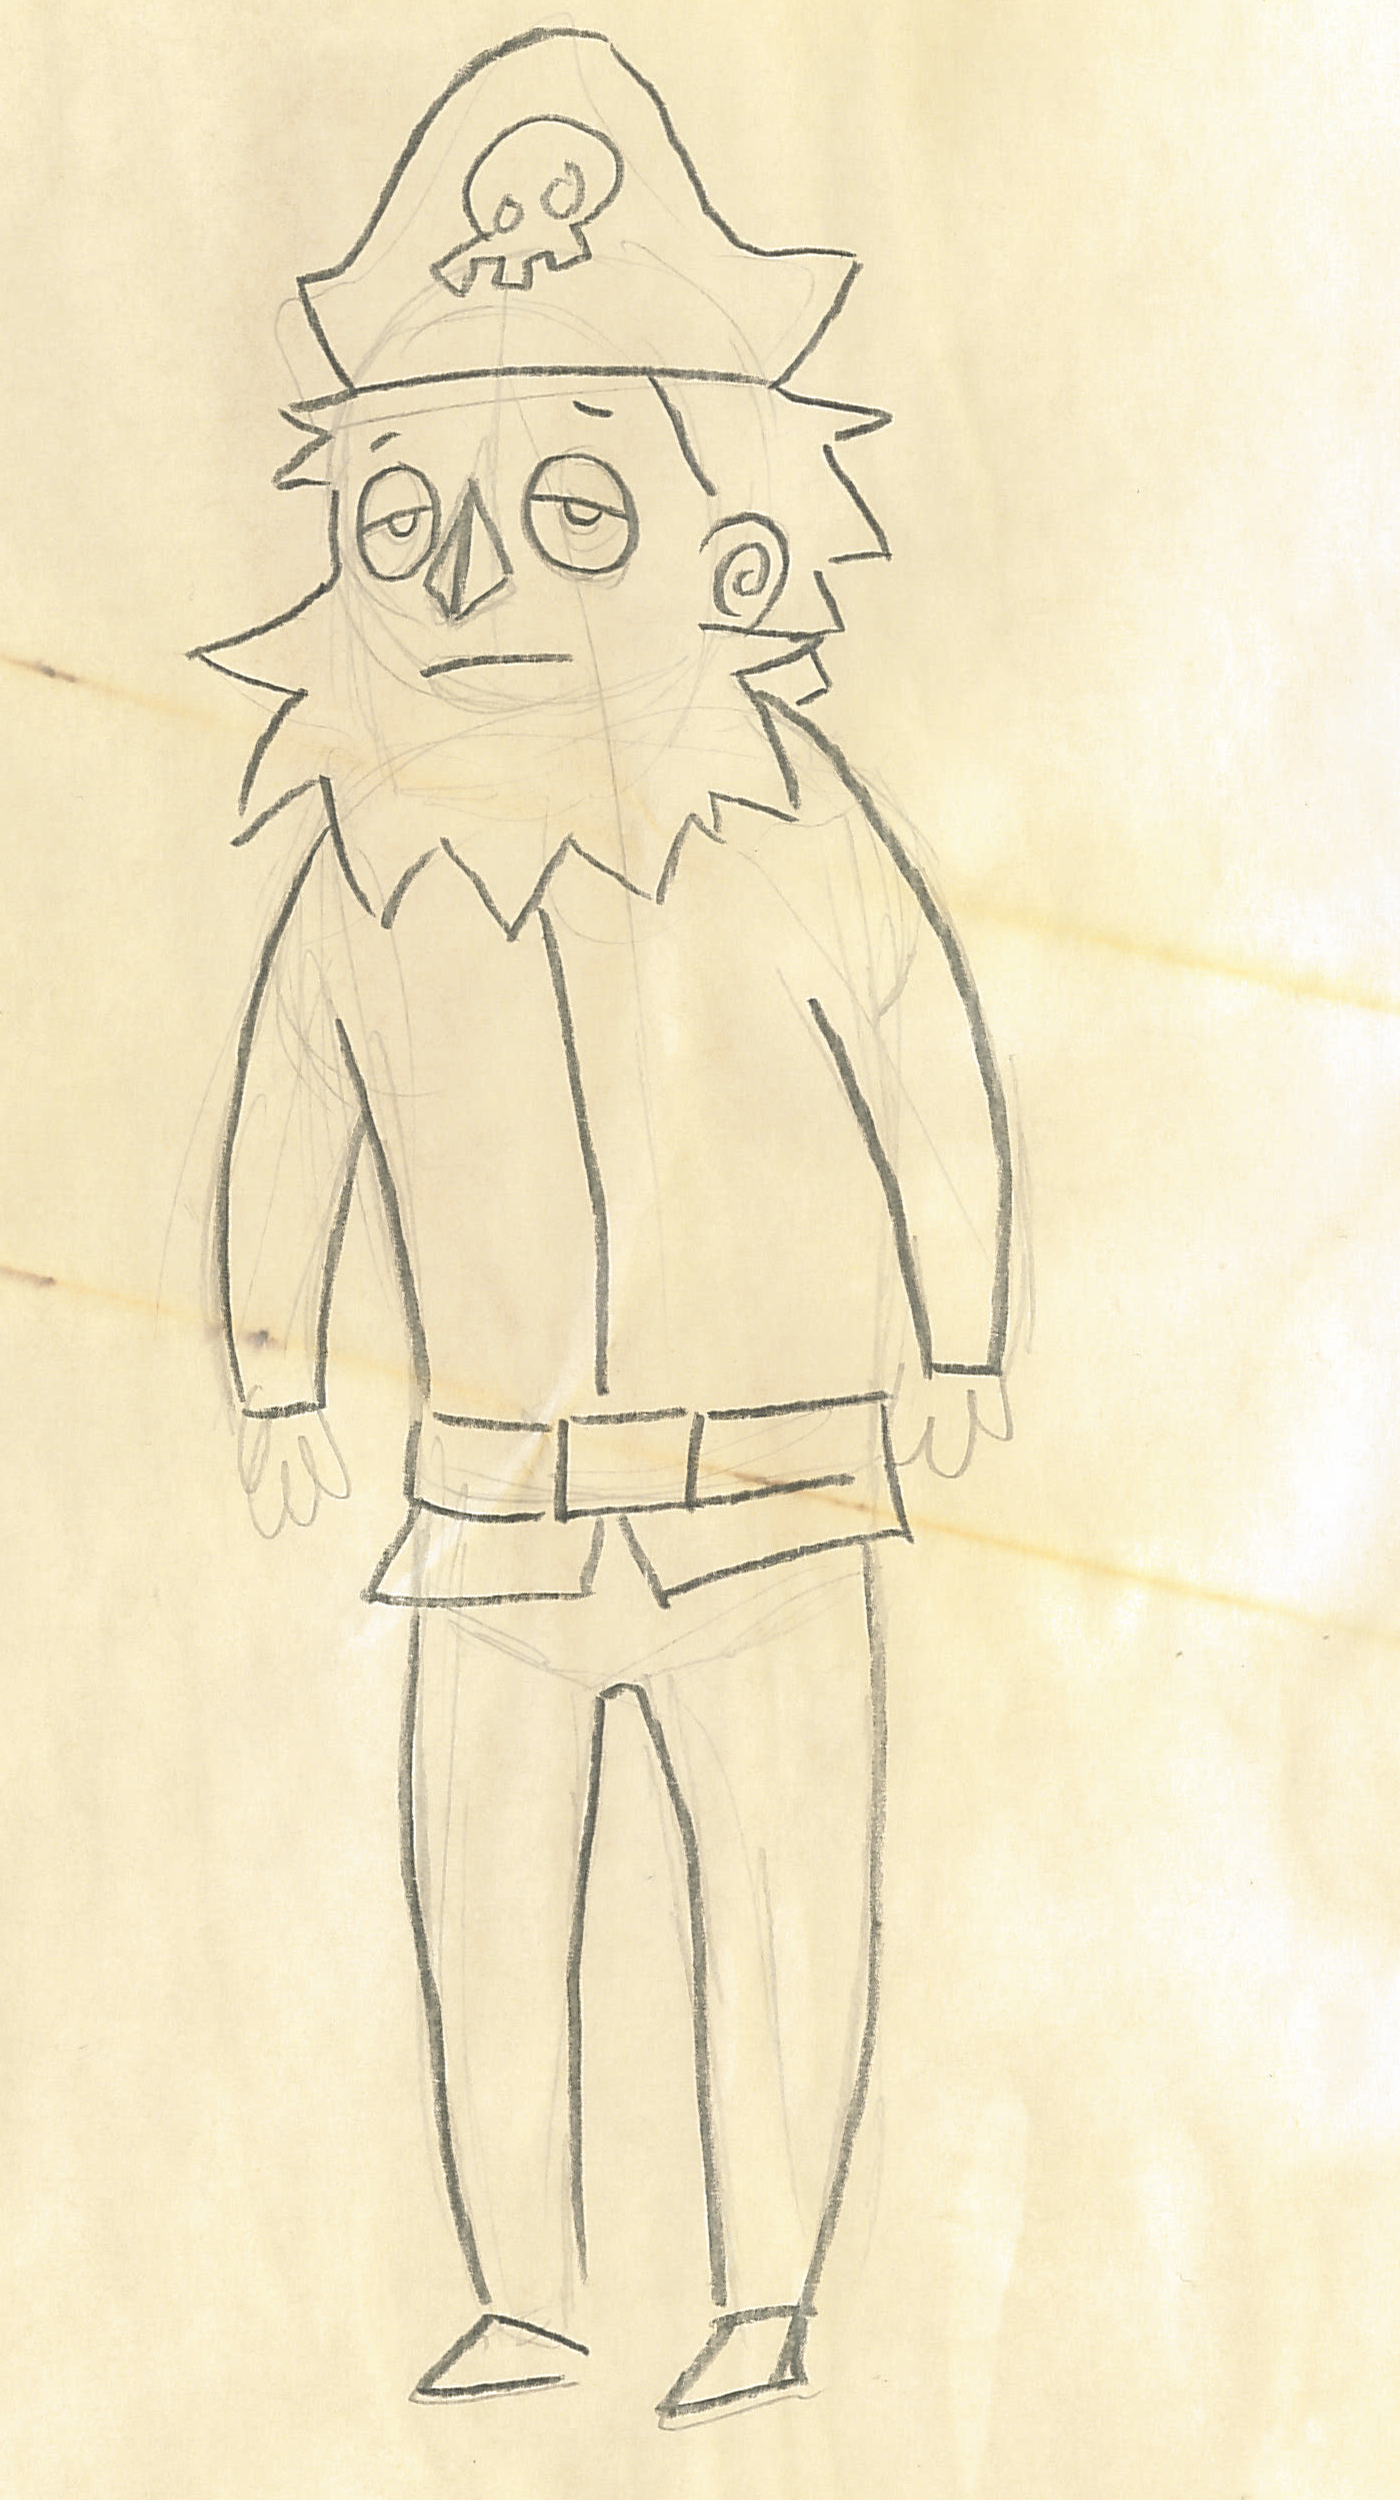
\includegraphics[width=\textwidth]{figures/pirate_concept_1.png}\caption{ \label{fig:pirate_concept_1}}
    \end{subfigure}
    \begin{subfigure}[b]{0.2\textwidth}
        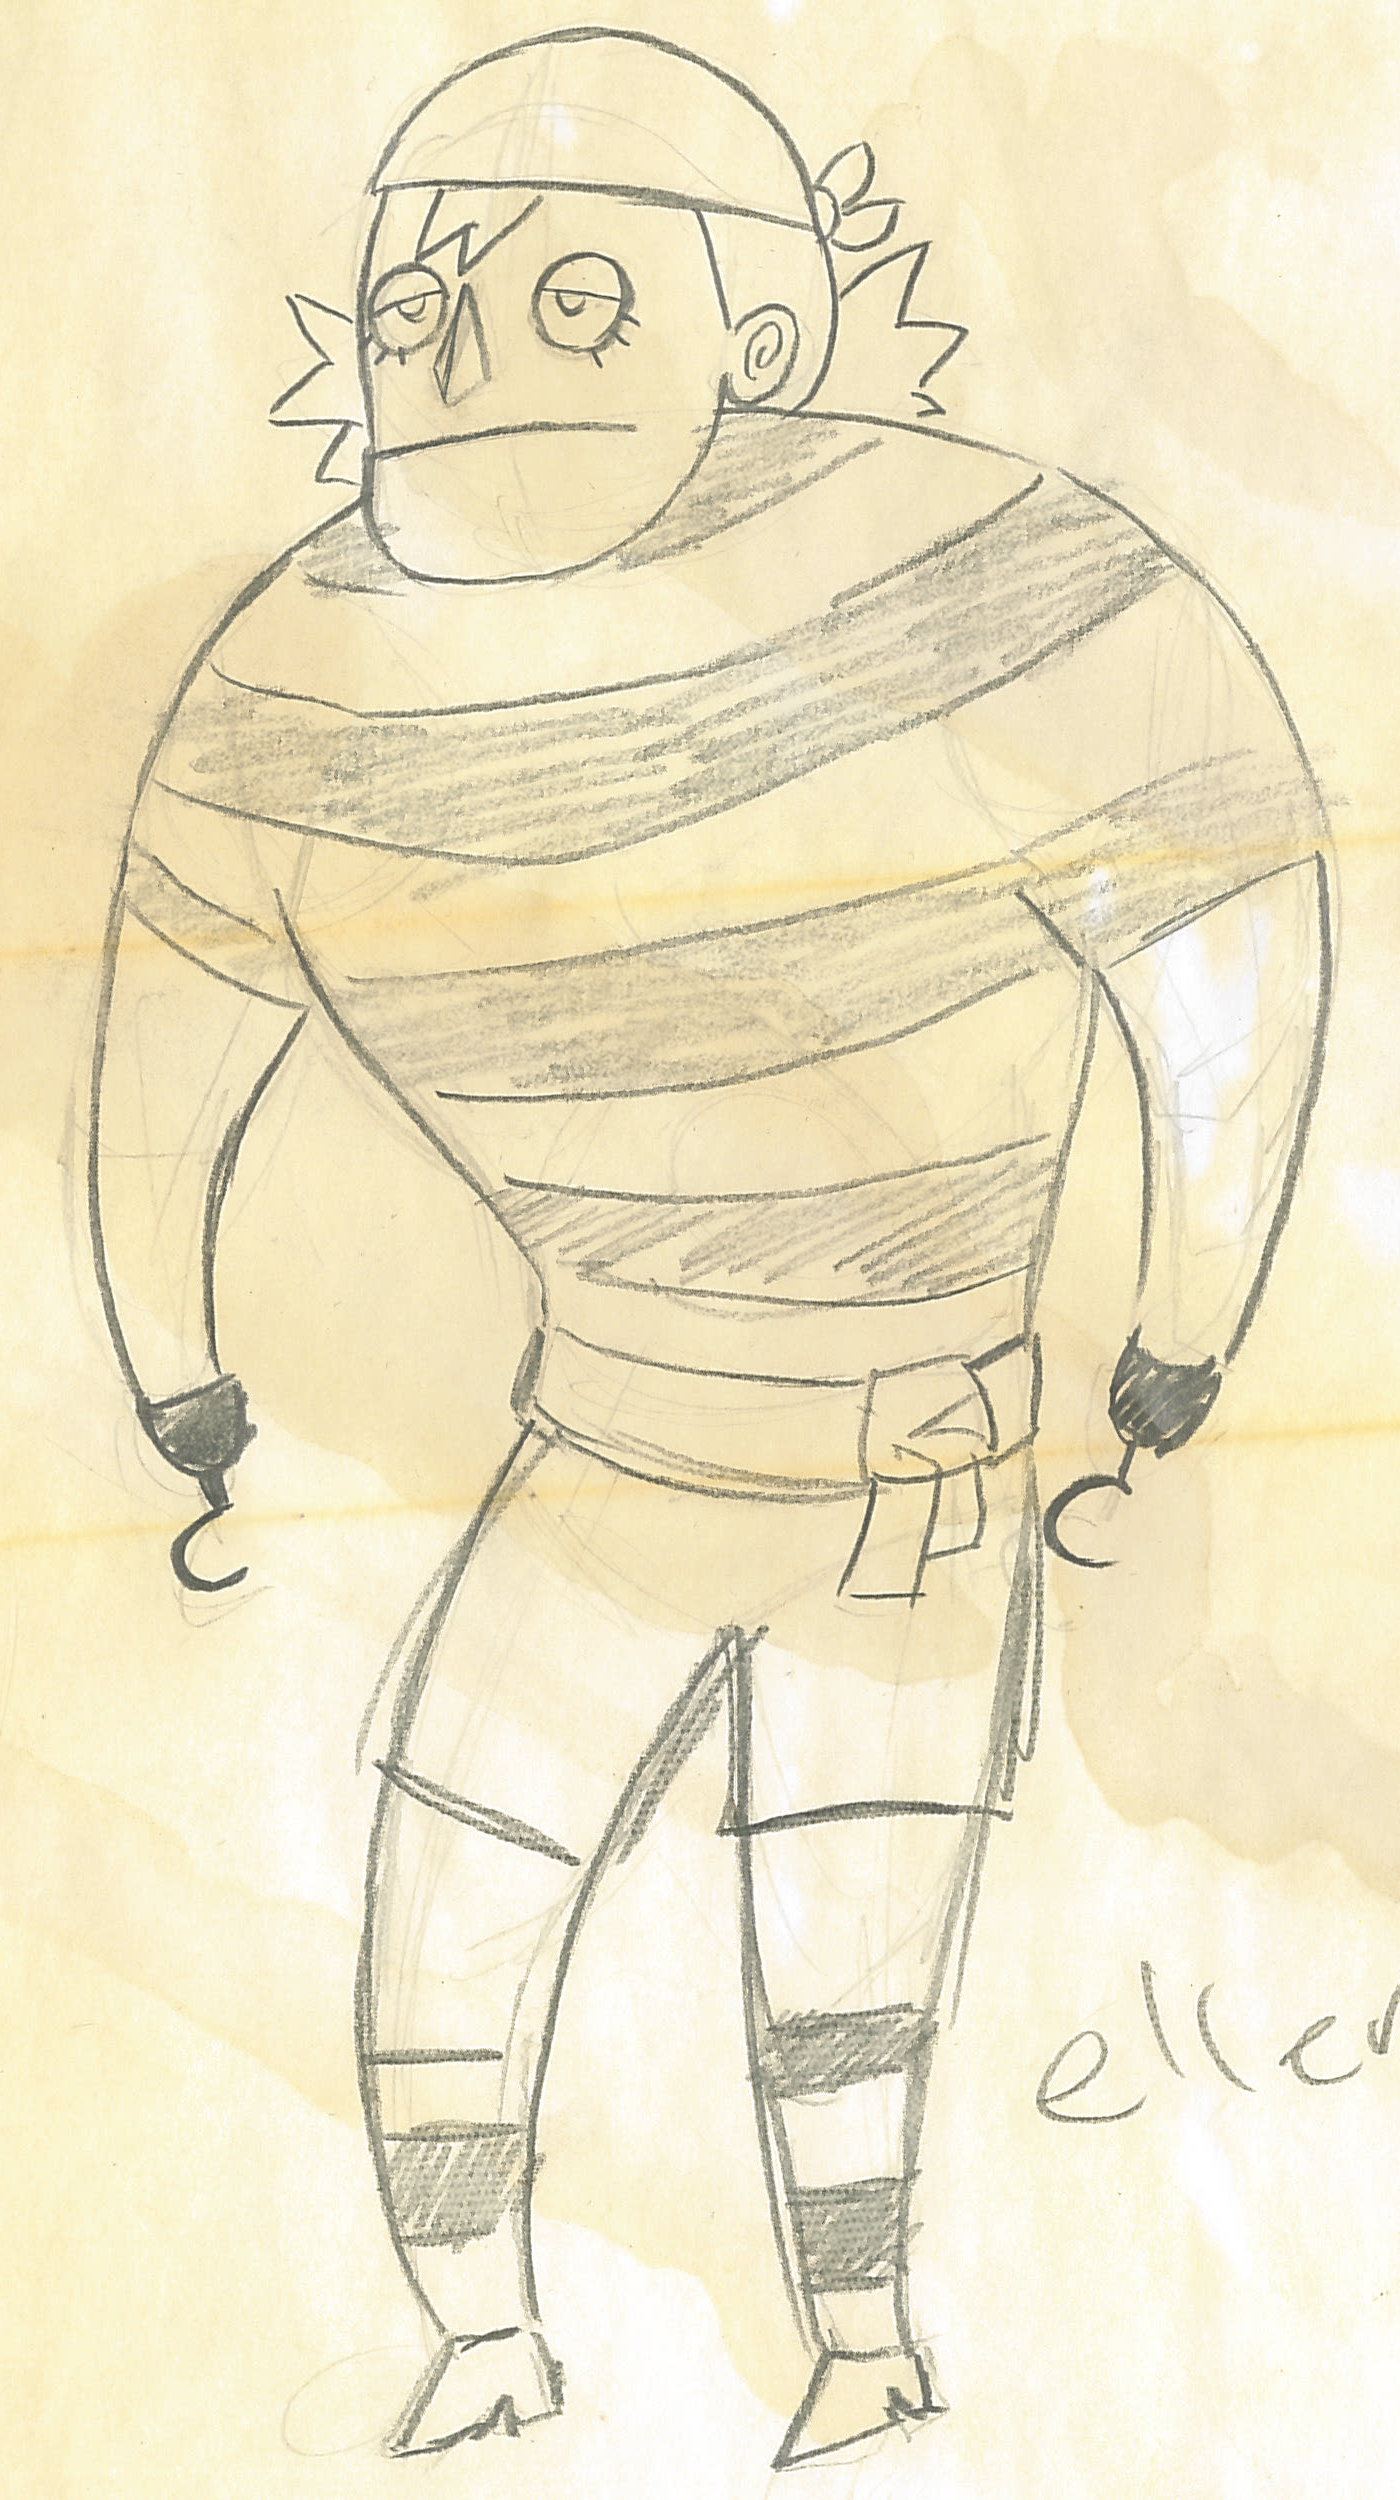
\includegraphics[width=\textwidth]{figures/pirate_concept_2.png}\caption{ \label{fig:pirate_concept_2}}
    \end{subfigure}
    \begin{subfigure}[b]{0.2\textwidth}
        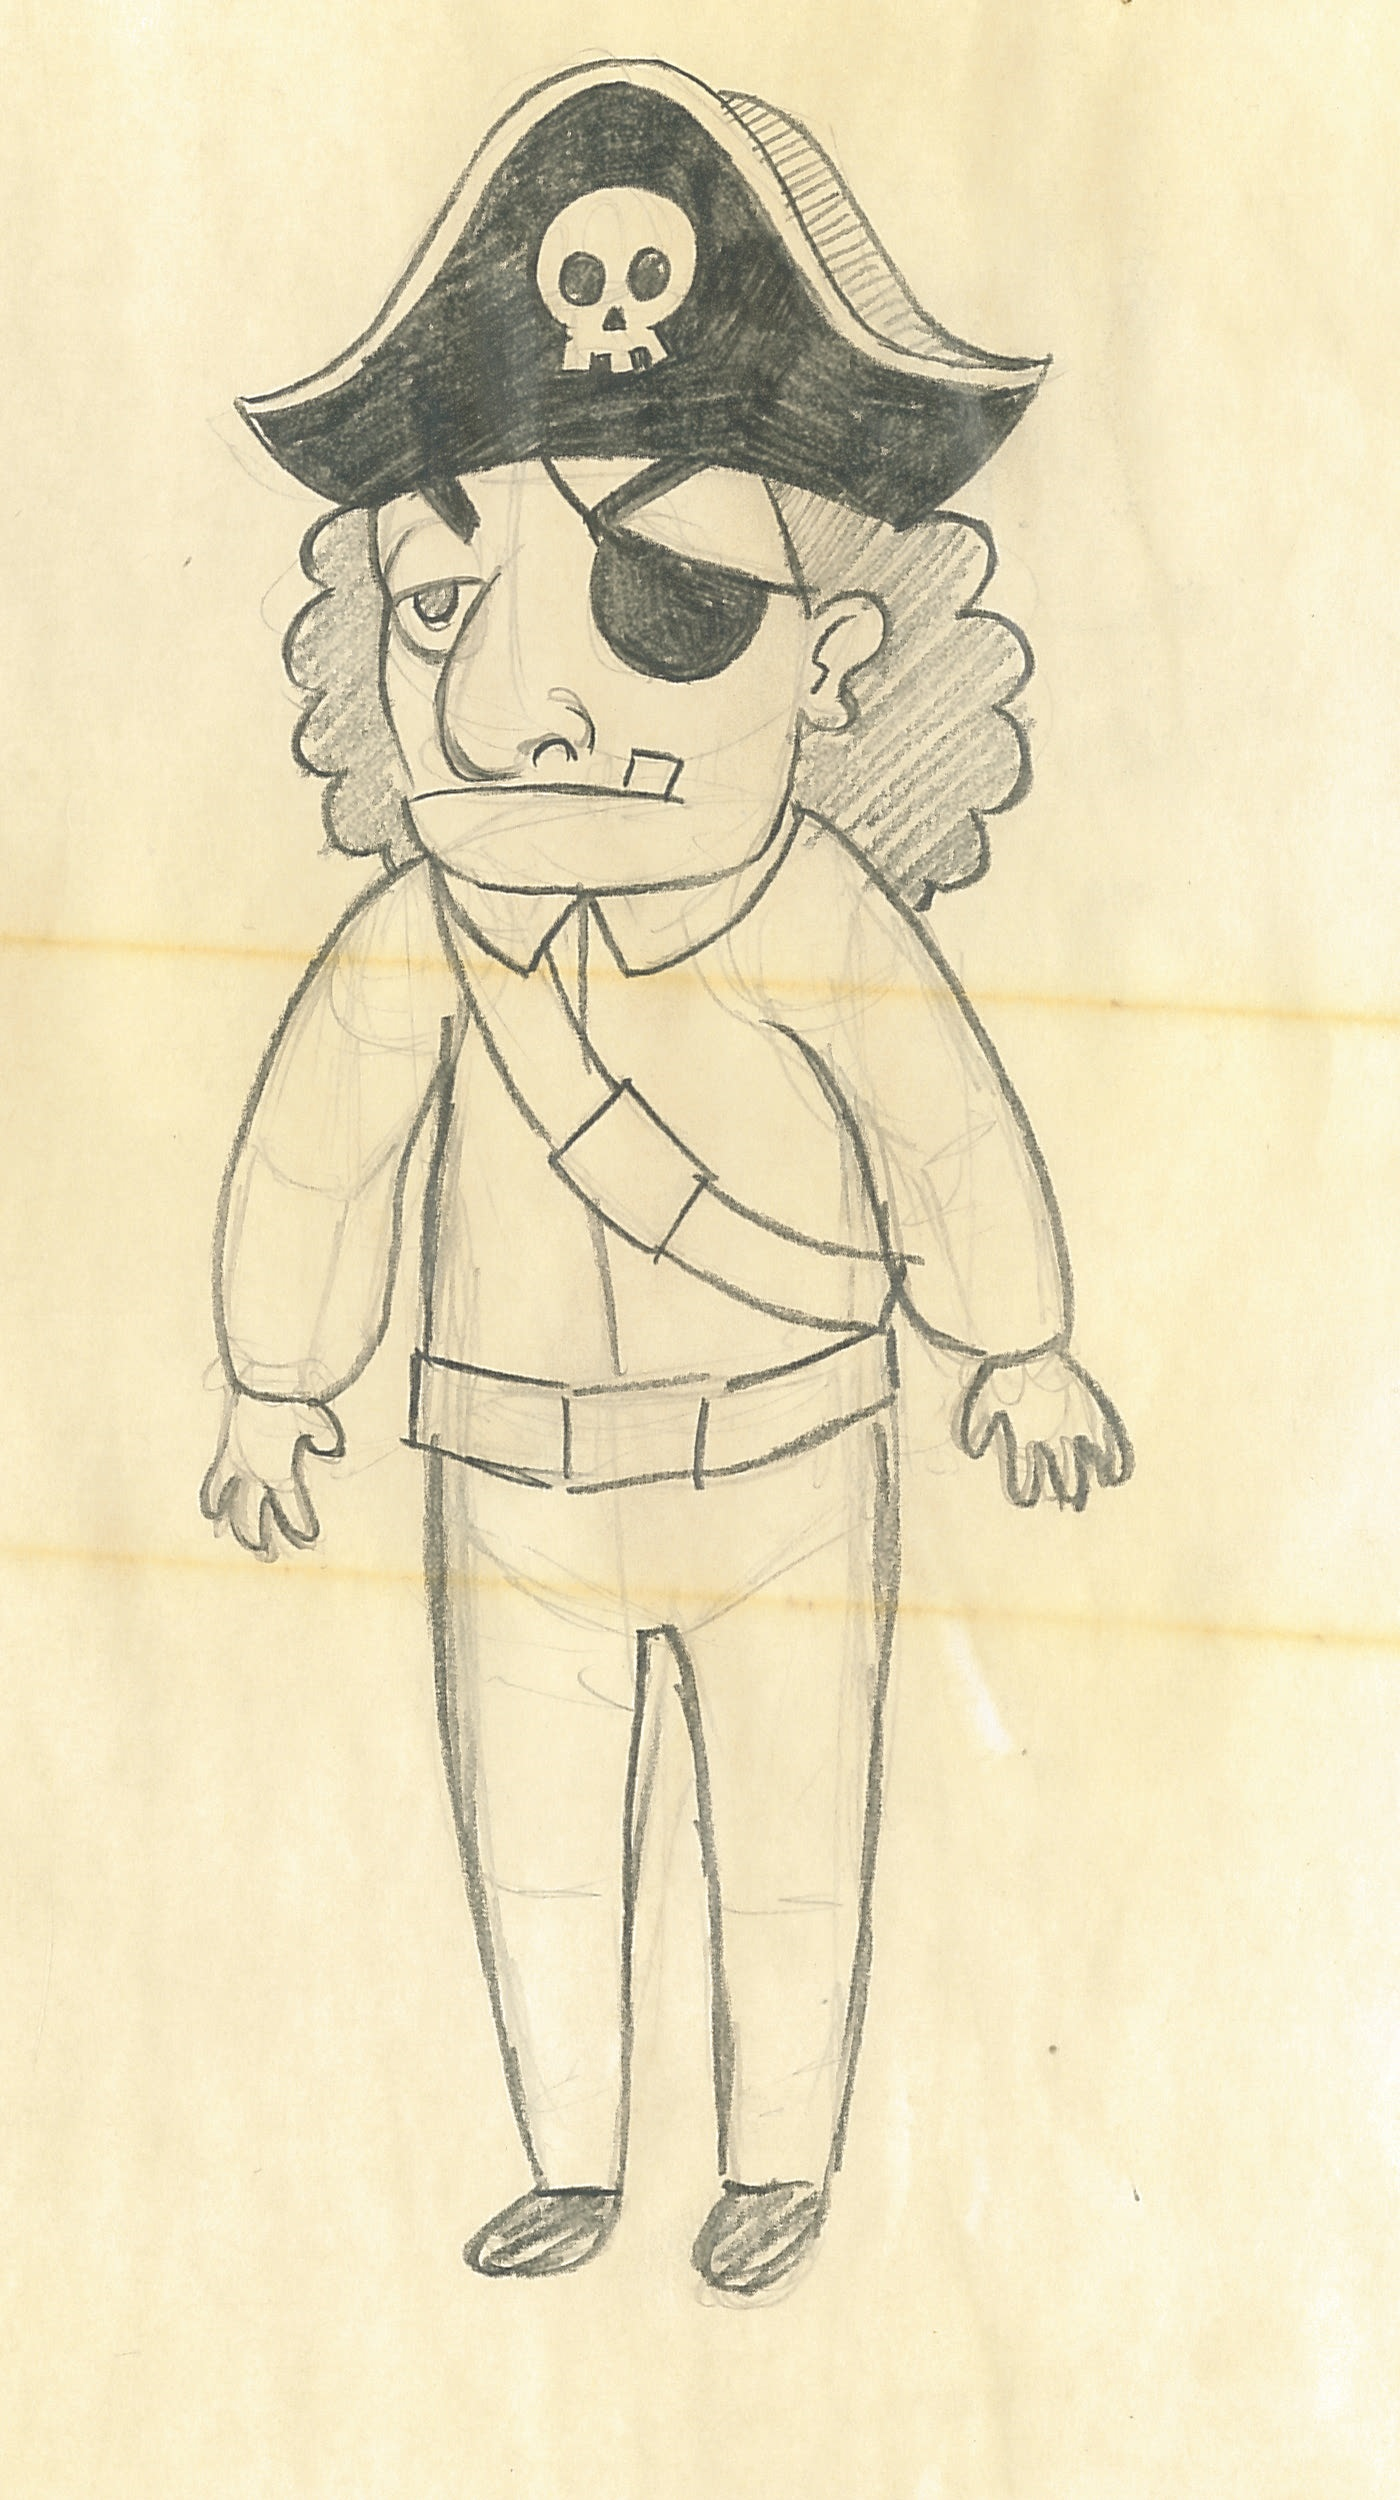
\includegraphics[width=\textwidth]{figures/pirate_concept_3.png}\caption{ \label{fig:pirate_concept_3}}
    \end{subfigure}
    \caption{Concept art of the pirate characters}\label{fig:pirate_concepts}
\end{figure}

In the end, the concept pictured in Figure \ref{fig:pirate_concept_2} was decided upon, in part due to its large torso; if the shirt and bandana are a certain colour, that colour will take up a relatively large percentage of the character's surface, allowing for it to be easily seen by the players, even when several characters are on the screen. 

\section{3D graphics}

\subsection{Modeling}
The models for this game are built and animated using Autodesk Maya, and consist of transformed primitives, such as spheres and cylinders. For example, the head of the player-controlled pirate characters is a transformed sphere, and the torso as well as the limbs consist of cylinders. The trunks of the palm trees are created from cylinders, and their leaves from planes. All four pirate characters have identical meshes, seen in Figure \ref{fig:pirate_mesh}.

\begin{figure}[h!]
	\centering
	\includegraphics[width=0.9\textwidth]{figures/pirate_mesh.png}
	\caption{Pirate mesh: front, side and back view \label{fig:pirate_mesh}}
\end{figure}

The components of the pirate mesh were transformed based on two reference images of the character design, assigned to two image planes, one showing a frontal view of the character, and one showing a side view. These planes can be seen in Figure \ref{fig:pirate_planes}. However, small changed were made during modeling, such as the short pigtails, which were changed intp longer braids in the final version.

\begin{figure}[h!]
	\centering
	\includegraphics[width=0.7\textwidth]{figures/pirate_planes.png}
	\caption{Pirate mesh: front, side and back view \label{fig:pirate_planes}}
\end{figure}

The interactive objects were not created using this technique, but rather modelled "free-hand". Like the character, the design of these objects aim for simplicity rather than realism.

\subsection{Textures}
Each pirate is assigned a \textit{lambert} material with a simple texture applied to it. The textures are very similar (simple face, light skin, neutrally coloured shorts), but they differ in the colour of each pirate's bandana and shirt colour. The colours of the four characters are red, green, yellow, and blue, as pictured in figure \ref{fig:pirate_rainbow}. The green colour specifically is chosen so that it is not too similar to the yellow colour --- the two were reviewed by a colour deficient person, who often has trouble discerning between light green and yellow colours. This person was able to easily discern between the yellow and green pirates.

\begin{figure}[h!]
	\centering
	\includegraphics[width=\textwidth]{figures/pirate_rainbow.png}
	\caption{All four player colours \label{fig:pirate_rainbow}}
\end{figure}

The texture was applied to the pirates using UV mapping; the geometry is flattened onto a two-dimensional coordinate system. Based on this flattened-out UV-map, an image containing all the necessary colours was created. An example of such a UV map (specifically for the red pirate) is seen in Figure \ref{fig:uv_map}.

\begin{figure}[h!]
	\centering
	\includegraphics[width=0.7 \textwidth]{figures/uv_map.png}
	\caption{The UV map for a pirate \label{fig:uv_map}}
\end{figure}